%
% Theory
%

% !TEX root = ../../main.tex

\chapter{Grundlagen}

\section{Natürliche Evolution vs. Artifical}

  Natürliche Evolution hat kein vordefiniertes Ziel und ist ein sogenannter open-ended Anpassungsprozess.
  Unter einem open-ended Anpassungsprozess in der natürlichen Evolution versteht man die Anpassung an die natürliche Umgebung.
  Da sich die natürliche Umgebung stetig ändert, ist der Prozess immer im Gange und endet nie.
  Artifizielle Evolution jedoch ist ein Optimierungsprozess,
  welcher versucht Lösungen zu vordefinierten Probleme zu finden~\cite[S.1]{book:bioInspired}.

  \subsection{Intelligent Design\label{sub:IntelligentDesign}}

    \todo[inline]{intelligent design}

\section{Artifical Evolution}

    \subsection{Individuum\label{sub:individual}}
      Als Individuum wird die zu evolvierende künstliche Kreatur bezeichnet.
      Ein Individuum hat einen zugehörigen Genotyp~(\vref{sub:genotyp}) und dessen Phänotyp~(\vref{sub:phenotyp}).
    \subsection{Genotyp\label{sub:genotyp}}
      Das genetische Material eines Individuums wird als Genotyp bezeichnet~\cite[S.5]{book:bioInspired}.
      Es beeinhaltet alle wichtigen Informationen zur Reproduktion des Individuums.
    \subsection{Genom\label{sub:genom}}
      Das Genom ist eine Repräsentation des Genotyps.
      Es beinhaltet nur reine Werte, jedoch keine Information was diese bedeuten.
      Erst durch den Geno- und Phäntoyp werden den Werten einen Sinn gegeben.

    \subsection{Phänotyp\label{sub:phenotyp}}
      Der Genotyp kann zu einem Phänotyp abgebildet werden.
      In einer künstlichen Umgebung (wie der Pixelwelt des Computers) kann man sagen,
      dass der Phänotyp die Pixelrepräsentation des Genotyps ist.
      Wenn der Genotyp die Länge und Breite eines Rechtecks beschreibt, so ist das grafisch gezeichnete Rechteck auf dem Monitor der Phänotyp~(\vref{fig:genoPheno}).
      \begin{figure}[H]
        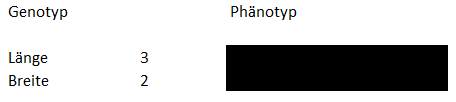
\includegraphics[scale=1]{graphics/genotyp_phenotyp}
        \caption{Genotyp und Phänotyp\label{fig:genoPheno}}
      \end{figure}

    %% in bioInspired wird genetic repärsentation erwähnt
    \subsection{Genetische Repräsentation}

    Der erste Schritt bei der Definition eines evolutionären Algorithmus ist die Auswahl der genetischen Repräsentation.
    Nicht alle Arten von evolutionären Algorithmen harmonieren mit jeder Repräsentation.
    Die genetische Repäsentation beschreibt die Elemente eines Genomes und wie diese in einen Phänotyp gemapped werden~\cite[S.16]{book:bioInspired}.

      \subsubsection{Diskrete Repräsentation\label{par:GeneticRepresentationDiscrete}}

        Bei der diskreten Repräsentation kann das Genom als binären String dargestellt [0111110] werden.
        Dieser binäre String kann anschliessend in einen Phänotyp übersetzt werden.
        Zum Beispiel kann eine Bitsequenz, direkt zu einer Zahl als Phänotyp übersetzt werden [0011] -> 3.
        Ebenfalls kann eine diskrete Repräsentation eine Folge von beliebigen Zeichen annehmen [ABCDEF].
        Wenn eine diskrete Repräsentation nur einzigartige Werte beinhaltet, spricht man von einer Sequenz.
        D. Floreano und C. Mattiussi bringen dazu ein gutes Beispiel anhand des Travelling Sales Man Problems an:
        Jeder Buchstabe in der Sequenz repräsentiert dabei einen Ort, welchen es zu besuchen gilt~(\vref{fig:travelling})~\cite[S.18]{book:bioInspired}.

        \begin{figure}[H]
          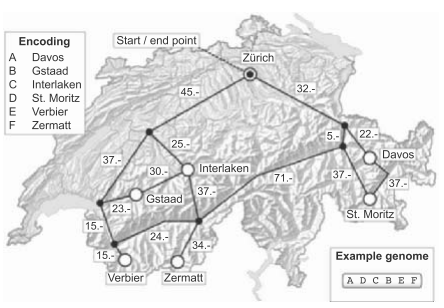
\includegraphics[scale=0.9]{graphics/discret_representation}
          \caption{Beispiel Diskrete Repräsentation \cite[S.18]{book:bioInspired} \label{fig:travelling}}
        \end{figure}

      \subsubsection{Reale-Werte-Repräsentation\label{par:GeneticRepresentationReal}}

        Weiter kann die Reale-Werte-Repräsentation gewählt werden.
        Das Genom~(\vref{fig:real_value_representation}) wird hierbei durch reelle Zahlen repräsentiert.
        Beispielsweisse kann die optimale Position eines Zimmers (beste Flächennutzung) in einem Haus
        durch reale Zahlen dargestellt werden.
        \begin{figure}[H]
          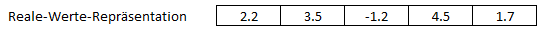
\includegraphics[scale=1]{graphics/real_value_representation}
          \caption{Beispiel Reale-Werte-Repräsentation \label{fig:real_value_representation}}
        \end{figure}

      \subsubsection{Baum-Repräsentationen\label{par:GeneticRepresentationTree}}

        Das zu evolvierende Objekt kann durch einen Baum dargestellt werden.
        \\
        Baum Repräsentationen (\vref{fig:baum}) werden eingesetzt um hierarchische Strukturen mit Verzweigungen und Bedingungen zu beschreiben~\cite[S.19]{book:bioInspired}.
        Baumstrukturen haben den Vorteil, dass sie sehr gut rekursiv durchlaufen werden können. Viele Probleme aus der Informatik lassen sich einfacher rekursiv als iterativ lösen.
        \begin{figure}[H]
          \Tree[.* [.+ [.2 ] [.7 ] ].+ [.- [.5 ] [.1 ] ] ].*
          \caption{Darstellung einer Rechnung als Baum\label{fig:baum}}
        \end{figure}

    \subsection{Initiale Population}
      Die Grösse der zu evolvierenden Population kann selber bestimmt werden.
      Jedoch muss beachtet werden, dass eine grössere Population mehr Rechenaufwand bedeutet.
      Auch die Eigenschaften des Suchraums dürfen dabei nicht ignoriert werden.
      Wichtig bei der Erstellung einer initialen Population ist, möglichst diverse~(\vref{sub:diversity}) Individuen zu generieren,
      damit nicht wertvolle Lösungen verspielt werden.

    \subsection{Fitness-Funktion}

      Mit Hilfe der Fitness-Funktion lassen sich Individuen beurteilen,
      wie gut geeignet ihre Gene sind um die Problemstellung zu bewältigen.
      In der natürlichen Evolution ist die Fitness des Tieres, wie viele Nachkommen es erzeugen kann.
      In der technischen Welt jedoch muss der Anwender sie jeweils selber definieren und
      nach seiner Problemstellung anpassen. Oft ist die evaluation der Fitness-Funktion
      die rechenintensivste Teilaufgabe eines evolutionären Algorithmus~\cite[S.22]{book:bioInspired}.

    \subsection{Diversität\label{sub:diversity}}
      Die Diversität einer Population von Individuen beschreibt wie verschieden die Individuen zueinander sind.
      Durch diese Kennzahl alleine lässt sich jedoch noch keine Aussage über die Diversität treffen.
      Erst wenn mehrere Generationen von Populationen vorhanden sind, kann diese Kennzahl benutzt werden um die Diversität zu beurteilen.
      Eine nummerisch grössere Zahl deutet darauf hin das die Individuen divers sind.



    \subsection{Selektionsoperation}

      Eine Selektionsoperation hilft einem möglichst gut geeignete Individuen einer Generation zu selektieren.
      Die Selektierten bilden die Basis für die nächste Generation.
      Eine grosse Herausforderung beim Selektieren ist die Erhaltung der Diversität.
      \subsubsection{Selektionsdruck}

        Als Selektionsdruck wird der Prozentsatz der Individuen der aktuellen Generation,
        welche man verwendet um Nachkommen zu erzeugen, bezeichnet.
        Ein hoher Selektionsdruck bedeutet das nur wenige Individuen zur Reproduktion selektiert werden~\cite[S.23]{book:bioInspired}.

      \subsubsection{Proportionale Selektion}

        Bei der proportionalen Selektion wählt man die Reproduktionsrate proportional zur Fitness.
        D. Floreano und C. Mattiussi~\cite[S.23]{book:bioInspired} beschreiben die Proportionale Selektion als Rouletterad,
        in dem jedes Individuum ein Stück des Rouletterad für sich beanspruchen~(\vref{fig:rouletteWheel}).
        Das Stück welches sie beanspruchen, ist so gross, wie ihre Fitness im Vergleich zu der Fitness ihrer Konkurrenten.
        Das Individuum mit der grössten Fitness wird auch das grösste Stück des Rouletterads für sich beanspruchen und hat somit die grösste Wahrscheinlichkeit Nachkommen zu erzeugen.
        Wenn die Population \(N\) Indivduen gross ist, wird das Rad \(N\) mal gedreht um die Nachkommen zu bestimmen.
        Proportionale Selektion funktioniert schlecht wenn alle Individuen sehr ähnliche Fitnesswerte aufweisen oder es nur wenige/einen Ausreisser gibt.
        Denn dann haben alle Individuen die gleiche Chance selektiert zu werden.

        \begin{figure}[H]
          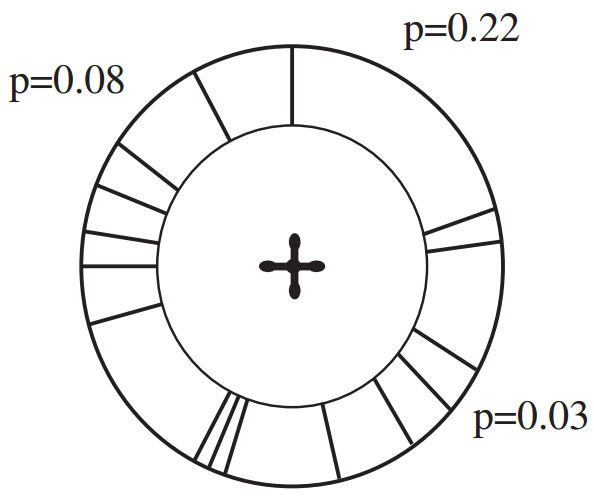
\includegraphics[scale=0.4, center]{graphics/roulettewheel}
          \caption{Rhouletterad der proportionalen Seleketion \cite[S.24]{book:bioInspired} \label{fig:rouletteWheel}}
        \end{figure}

      \subsubsection{Rang-basierte Selektion}

        Es wird zuerst eine Rangliste nach Fitness erstellt und dann werden die Reproduktionswahrscheinlichkeiten proportional zum Rang zugeordnet.
        Anstatt das Rouletterad~(\vref{fig:rouletteWheel}) nach Fitness der Individuen zu unterteilen, wird es anhand des Ranges unterteilt.
        Diese Selektionsstrategie hat den Vorteil gegenüber der proportionalen Selektion,
        dass die Fitness der Indivdueen ähnlich sein darf, jedoch wird mit hoher Wahrscheinlichkeit immer noch das besere selektiert werden.

      \subsubsection{Gekürzte Rang-basierte Selektion}

        Es wird eine Rangeliste wird für die Individuen der Population erstellt.
        Anstatt alle Individuen zu berücksichtigen werden nur die besten der Rangliste selektiert und diese produzieren Nachkommen (\vref{fig:truncated_rank_based_selection}).

        \begin{figure}[H]
          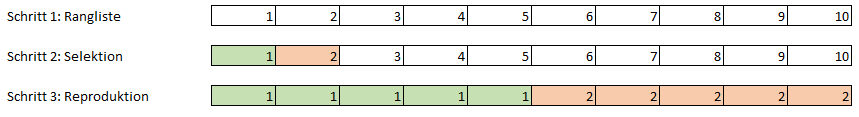
\includegraphics[scale=0.7, center]{graphics/truncated_rank_based_selection}
          \caption{Schritte einer gekürzten rang-basierten Selektion \label{fig:truncated_rank_based_selection}}
        \end{figure}


      \subsubsection{Turnier-basierte Selektion\label{par:Turnier}}

        Es werden \(k\) zufällig ausgewählte Individuen selektiert, diese Individuen tragen untereinander ein Turnier (\vref{fig:tournament_based}) aus.
        Das Turnier gewinnt jenes Individuum, welches den höchsten Fitnesswert aufweist.
        Dies wird solange wiederholt bis man wieder so viele Nachkommen hat,
        wie die Ursprüngliche Generation Individuen hatte.
        Ein grosser Vorteil von Turniert-basierter Selektion ist die gute Balance zwischen
        Selektionsdruck und genetischer Diversität, da alle Individuen in der Population die gleiche Wahrscheinlichkeit haben, für das Turnier selektiert zu werden.
        Somit können auch Indivduen mit niedrigem Fitnesswert ein Turnier gewinnen.

        \begin{figure}[H]
          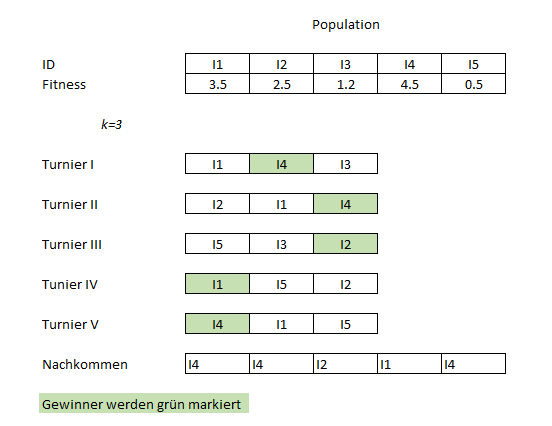
\includegraphics[scale=1, center]{graphics/tournament_based}
          \caption{Turnier-basierte-Selektion \label{fig:tournament_based}}
        \end{figure}

    \subsection{Rekombinationsfunktion}

        Bei der Rekombination werden jeweils zwei Individuen selektiert und
        deren Gen-Paare werden rekombiniert (untereinander vertauscht).
        \vref{fig:crossOver} veranschaulicht diesen Prozess.
        Nicht bei jedem Typ von evolutinären Algorithmen~(\vref{sub:artenEvAlgos}) und jeder Problemstellung ist Rekombination sinnvoll.
        Man nehme das Beispiel von einem Haus: Die Gene der Türen mit den Genen der Fenster zu vertauschen, ergibt keinen Sinn.


        \begin{figure}[H]
          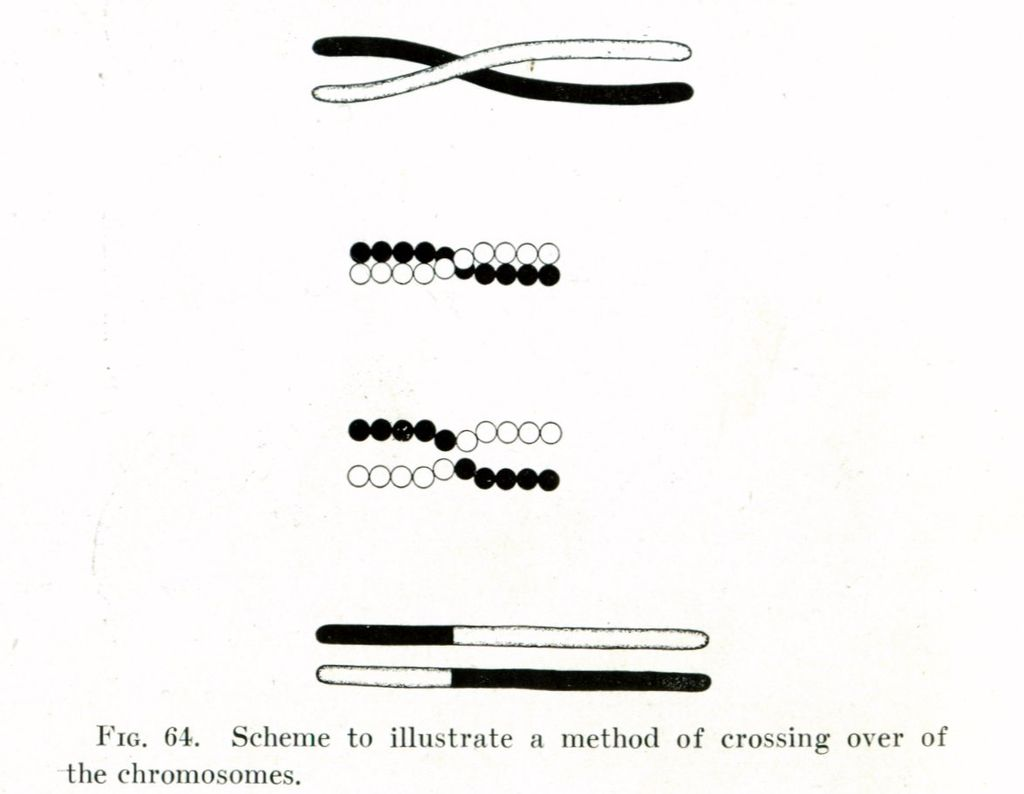
\includegraphics[scale=0.3, center]{graphics/morgan_crossover}
          \caption{Illustration des Crossover \cite[]{WikipediaEN:crossOver} \label{fig:crossOver}}
        \end{figure}

        \subsubsection{One-Point Crossover}

        Es wird ein zufälliger Cross-Over Punkt bestimmt an dem die Gene des Paares vertauscht werden (a)~\vref{fig:crossTypes}.
        Anwendbar ist diese Strategie bei Diskreten- und Realen-Werten-Repräsentationen.

        \subsubsection{Multi-Point Crossover}

          Funktioniert gleich wie One-Point Crossover, jedoch werden mehrere Punkte bestimmt und
          zwischen diesen Punkten werden dann die Gene ausgetauscht.

        \subsubsection{Uniform Crossover}

          Die Gene werden an \(n\) zufälligen Stellen vertauscht ( b) \vref{fig:crossTypes}).

        \subsubsection{Arithmetic Crossover}

          Der Durschnitt von den Genen an \(n\) zufälligen Positionen wird gebildet.
          Aus diesem Durchschnitt wird dann ein Nachkomme erzeugt ( c) \vref{fig:crossTypes}).
          Da arithmetische Operationen nur auf Zahlen anwendbar sind,
          kann dieser Crossover nur bei Reale-Werte-Repräsentationen verwendet werden.

        \subsubsection{Sequenzen}

          Bei Sequenzen gilt es die Regel zu erhalten, dass alle Einträge nur einmal vorkommen dürfen.
          Es wird ein Multi-Point Crossover durchgeführt unter Einhaltung der oben genannten Regel ( d) \vref{fig:crossTypes}).

        \subsubsection{Bäume}

        Bei Bäumen wird ein zufälliger Teil des Baumes, mit einem anderen Teil eines Baumes, von einem fremden Individuum vertauscht ( e) \vref{fig:crossTypes}).

        \begin{figure}[H]
          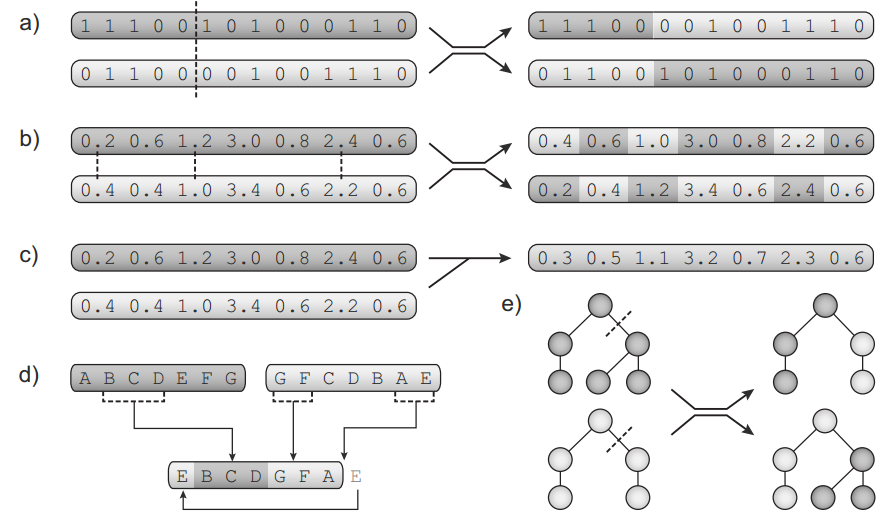
\includegraphics[scale=0.7, center]{graphics/crossover_types}
          \caption{Typen von Crossovers\cite[S.27]{book:bioInspired} \label{fig:crossTypes}}
        \end{figure}


    \subsection{Mutationsfunktion}

      Mutationen operieren auf dem Genotyp des Individuums.
      Die Positionen eines Genoms werden mit einer bestimmten Wahrscheinlichkeit \(p_{m}\) mutiert.
      Es ist jedoch Vorsicht geboten, da gewisse Lösungen durch Mutationen verloren gehen können.
      Darum sollten Mutationswahrscheinlichkeiten klein gewählt werden, da sonst keine gewinnbringende Evolution statt finden kann.

      \subsubsection{Binäre Repräsentationen}

        Wenn die Repräsentation aus binären Werten besteht, werden die Bits invertiert (oder nur bestimmte Segmente).
        Invertieren bedeutet, dass aus einem 0 eine 1 wird und umgekehrt (\vref{fig:mutation_binary_flip}).

        \begin{figure}[H]
          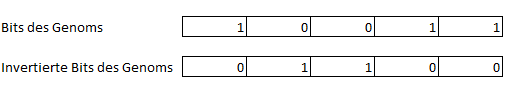
\includegraphics[scale=1, center]{graphics/mutation_binary_flip}
          \caption{Invertieren der Bits \label{fig:mutation_binary_flip}}
        \end{figure}

      \subsubsection{Reale-Werte-Repräsentationen}

        Bei Realen-Werte-Repräsentation wird jeweils zu einem bestehnden Wert ein nummerischer Wert addiert.
        Der Wert sollte zufällig berechnet werden. Die Zufallsfunktion welche dafür verwendet wird, sollte normalverteilt sein.
        Ebenfalls sollten der Zufallsfunktion Grezen angegeben werden, innerhalb deren sie Zahlen generiert (\vref{fig:mutation_real_value}).

        \begin{figure}[H]
          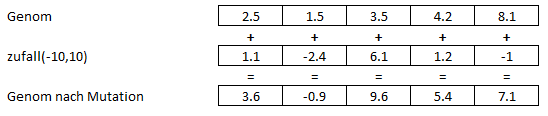
\includegraphics[scale=1, center]{graphics/mutation_real_value}
          \caption{Mutation von Reale-Werte-Repräsentationen \label{fig:mutation_real_value}}
        \end{figure}

      \subsubsection{Sequenzen}

        Zufällig ausgewählte Positionen der Sequenz werden miteinander vertauscht (\vref{fig:mutation_sequences}).

        \begin{figure}[H]
            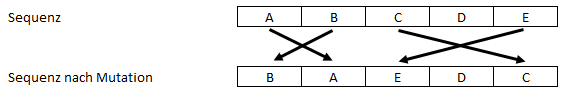
\includegraphics[scale=1, center]{graphics/mutation_sequences}
            \caption{Mutation von Reale-Werte-Repräsentationen \label{fig:mutation_sequences}}
        \end{figure}

      \subsubsection{Baum}

        Bei Bäumen werden Teilabschnitte mutiert.
        \begin{figure}[H]
            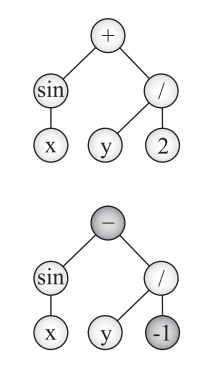
\includegraphics[scale=0.8, center]{graphics/mutation_tree}
            \caption{Mutation von Bäumen \cite[S.29]{book:bioInspired} \label{fig:mutation_tree}}
        \end{figure}


  \subsection{Arten von evolutionären Algorithmen\label{sub:artenEvAlgos}}

    Es gibt verschiedene Typen von evolutionären Algorithmen, welche sich hauptsächlich in der Wahl ihrer genetischen Repräsentation
    und Operationen unterscheiden~\cite{book:introEvComp}.
    Die Auswahl des evolutionären Algorithmus hängt von den Eingeschaft der Problemstellung ab.
    Es gibt keinen Algorithmus der alle Probleme optimal lösen kann~\cite{book:genAlgoDataStructsEvProg}.
    Die am häufigst verbreiteten Algorithmen sind: genetische Algorithmen~(\vref{item:genAlgo}),
    genetische Programmierung~(\vref{item:genProg}), evolutionäre Programmierung~(\vref{item:evProg})
    und evolutionäre Strategien~(\vref{item:evStrat}).

    \subsubsection{Genetische Algorithmen\label{item:genAlgo}}

      Die Genetischen Algorithmen~\cite{book:adapNaturalArtSys} arbeiten mit binären genetischen Repräsentationen.
      Es wird sowohl Rekombination als auch Mutation eingesetzt.

    \subsubsection{Genetische Programmierung\label{item:genProg}}

      Bei der genetischen Programmierung~\cite{book:genProg} werden Bäume als Repräsentation des Genoms eingesetzt. Wie bei den Genetischen Algorithmen,
      wird auch Rekombination und Mutation eingesetzt.

    \subsubsection{Evolutionäre Programmierung\label{item:evProg}}

      Bei der evolutionären Programmierung~\cite{book:artIntSimEv} wird ausschliesslich Mutation und keine Rekombination eingesetzt.
      Das Genom wird durch reale Werte repräsentiert. Als Selektionsoperator wird oft Turnier-basierte Selektion eingesetzt.

    \subsubsection{Evolutionäre Strategien\label{item:evStrat}}

      Evolutinäre Strategien~\cite{book:evStrat} sind ähnlich wie evolutionäre Programmierung.
      Die Varianz der Verteilung welche für die Mutation gebraucht wird, ist genetisch codiert.
